\documentclass{beamer}
\usepackage[italian]{babel}
\usepackage[utf8]{inputenc}
\usetheme{Berlin}
\usecolortheme{wolverine}
\usepackage{booktabs}
\usepackage{siunitx}
\usepackage{graphicx} 
\usepackage{amsmath}
\usepackage{caption}
\usepackage[italian]{babel}
%\usepackage[utf8]{inputenc
\usepackage[absolute,overlay]{textpos}
\usepackage{multirow}
\usepackage{subfig}


\title{WAVEMETER}
\subtitle{Caratterizzazione di due misuratori di lunghezza d'onda e loro applicazioni}

\author{S.~Bottaro\inst{1} \and L.M.~Perrone\inst{1}}

\institute[Unipi] % (optional, but mostly needed)
{
  \inst{1}%
  Dipartimento di Fisica\\
  Università di Pisa
  }
  
\date{Seminario - 2016}  

\AtBeginSubsection[]
{
  \begin{frame}<beamer>{Outline}
    \tableofcontents[currentsection,currentsubsection]
  \end{frame}
}

\begin{document}


\begin{frame}{Gamut}
\begin{figure}
\centering
\label{fig:8_CIExy1931_sRGB_gamut_D65}
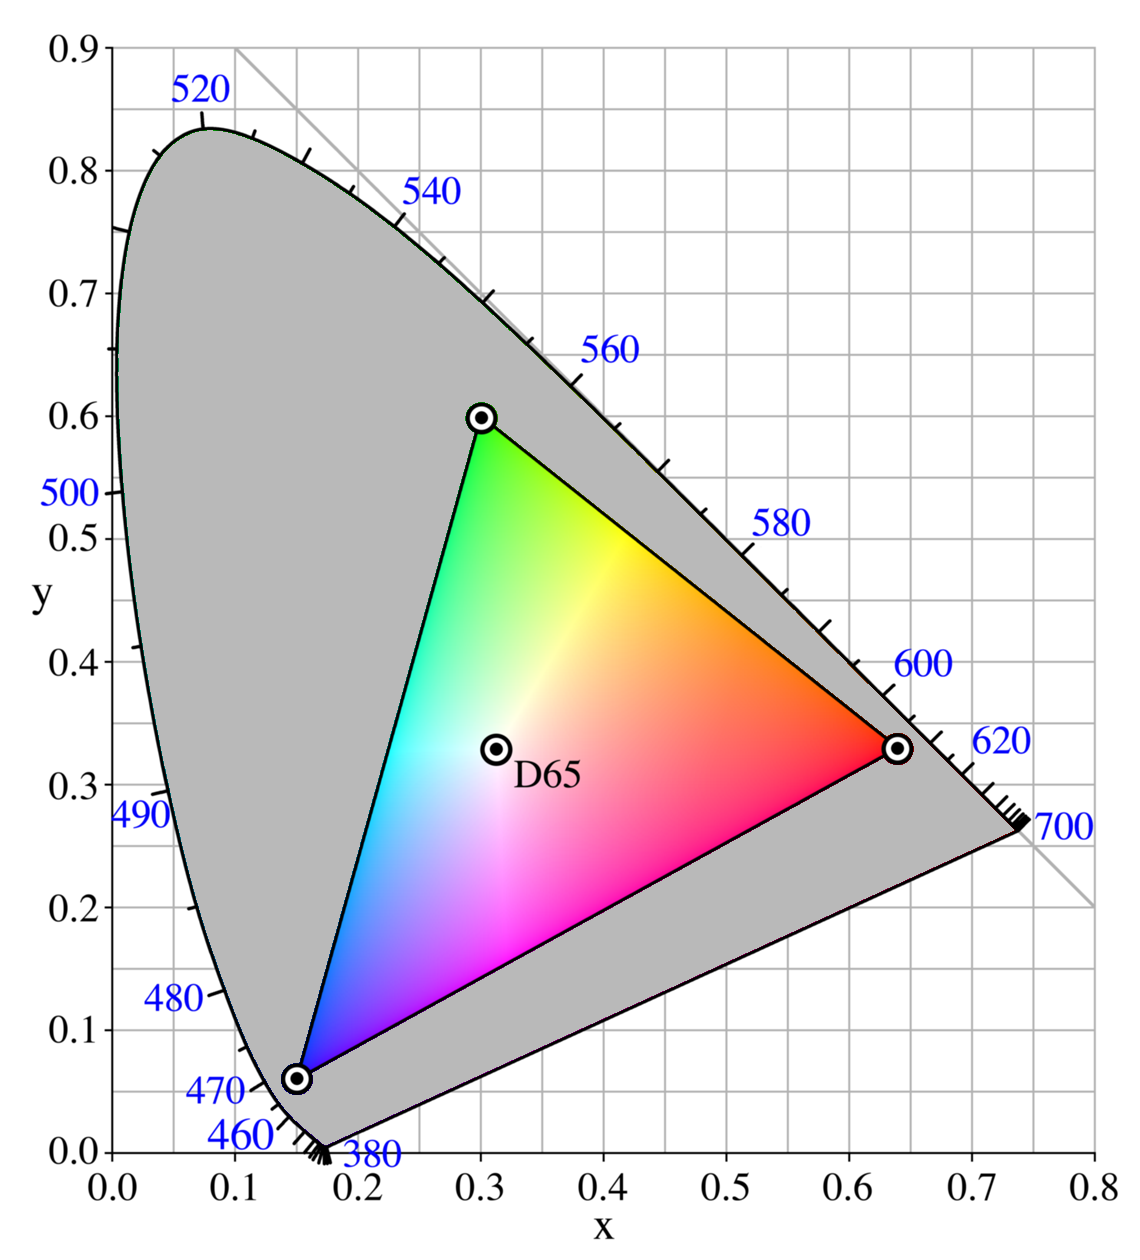
\includegraphics[width=0.55\linewidth]{./8_CIExy1931_sRGB_gamut_D65}
\end{figure}
\end{frame}

\begin{frame}{Tristimulus Functions}



\begin{textblock}{12}(-1.5,4)
\begin{figure}
\centering
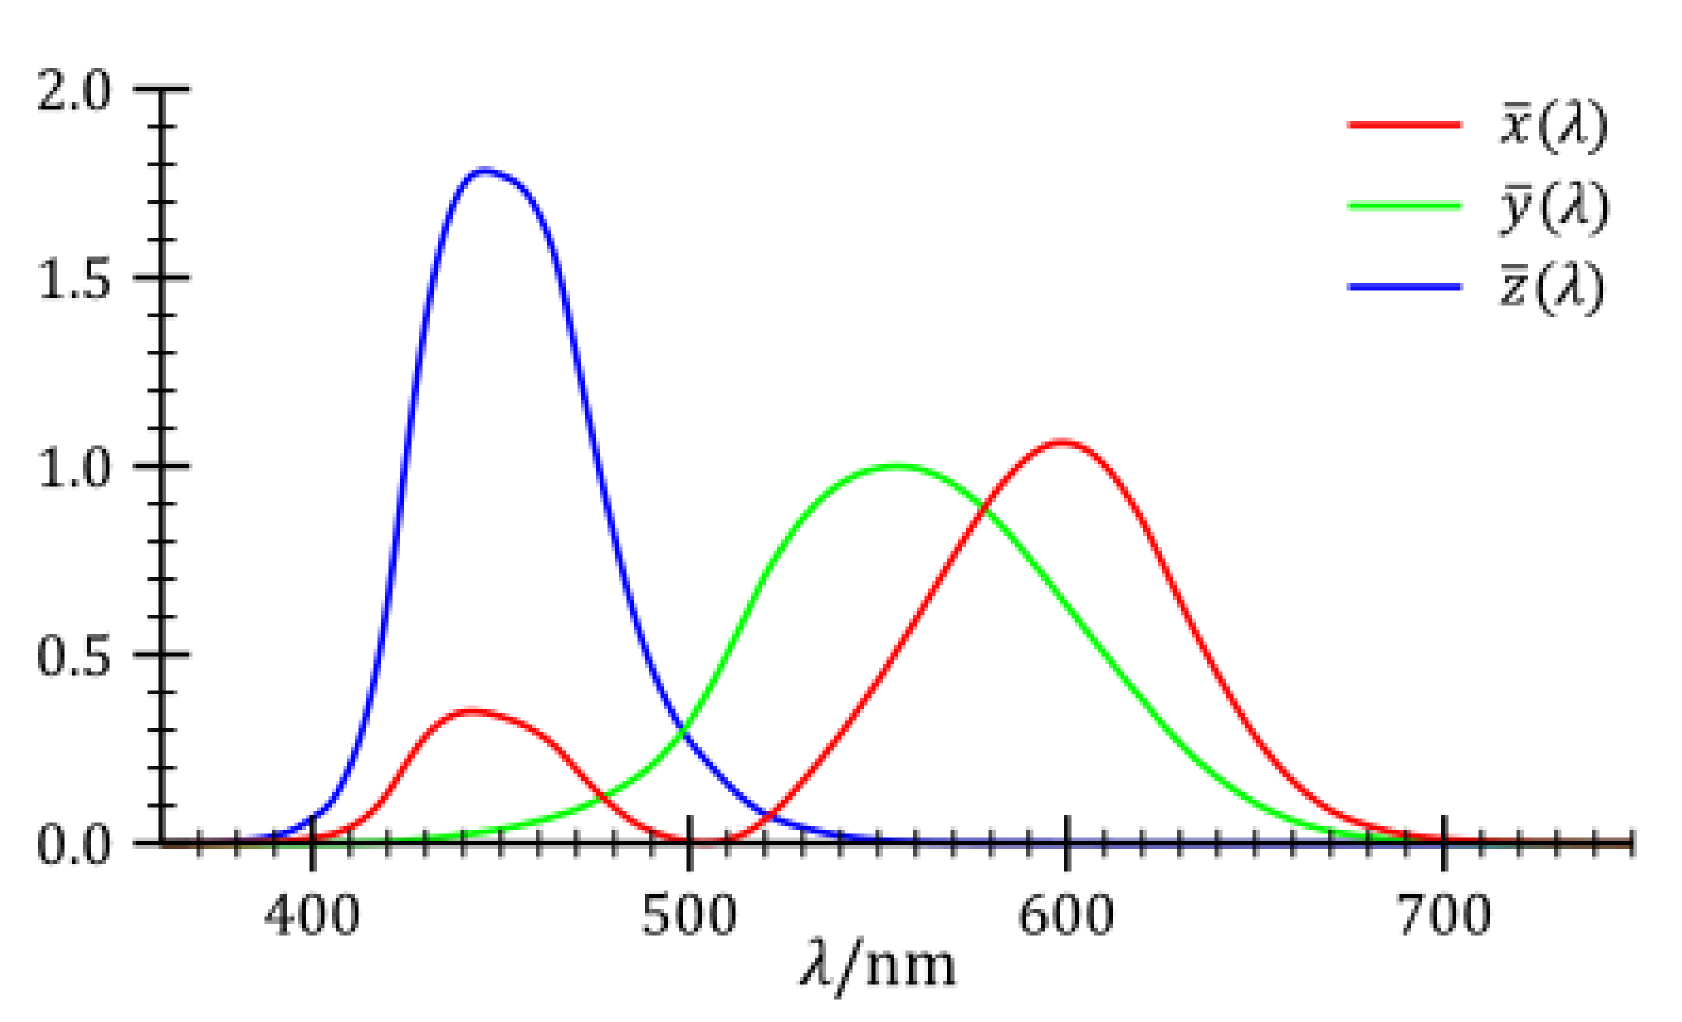
\includegraphics[width=0.7\linewidth]{./match_fun}
\label{fig:446px-CIE_1931_XYZ_Color_Matching_Functions}
\end{figure}
\end{textblock}


\begin{textblock}{8}(7,4)
\begin{equation}
\mathrm{X} = \int_{380}^{780} M(\lambda) \bar{x}(\lambda) \mathrm{d} \lambda
\end{equation}

\begin{equation}
\mathrm{Y} = \int_{380}^{780} M(\lambda) \bar{y}(\lambda) \mathrm{d} \lambda
\end{equation}

\begin{equation}
\mathrm{Z} = \int_{380}^{780} M(\lambda) \bar{z}(\lambda) \mathrm{d} \lambda
\end{equation}
\end{textblock}

\end{frame}

\begin{frame}{Luminosity Function - X}

\begin{itemize}
\item $\bar{x}(\lambda)$, $\bar{y}(\lambda)$ e $\bar{z}(\lambda)$ si definiscono \emph{colour matching functions}. 
\item Le colour matching functions sono definite in modo tale da riprodurre la responsività dei tre tipi di coni presenti nell'occhio.
\item In particolare la $\bar{y}(\lambda)$ è detta \textit{luminosity function}: descrive la sensitività spettrale media della percezione visuale della luminosità (da parte dell'occhio umano).
\item Qualitativamente la tristimulus function X (definita prima) rappresenta la percentuale di rosso che compone la radiazione incidente. 
\end{itemize}
\end{frame}

\begin{frame}{Cella fotovoltaica}
\begin{figure}
\centering
\label{fig:dati_normal}
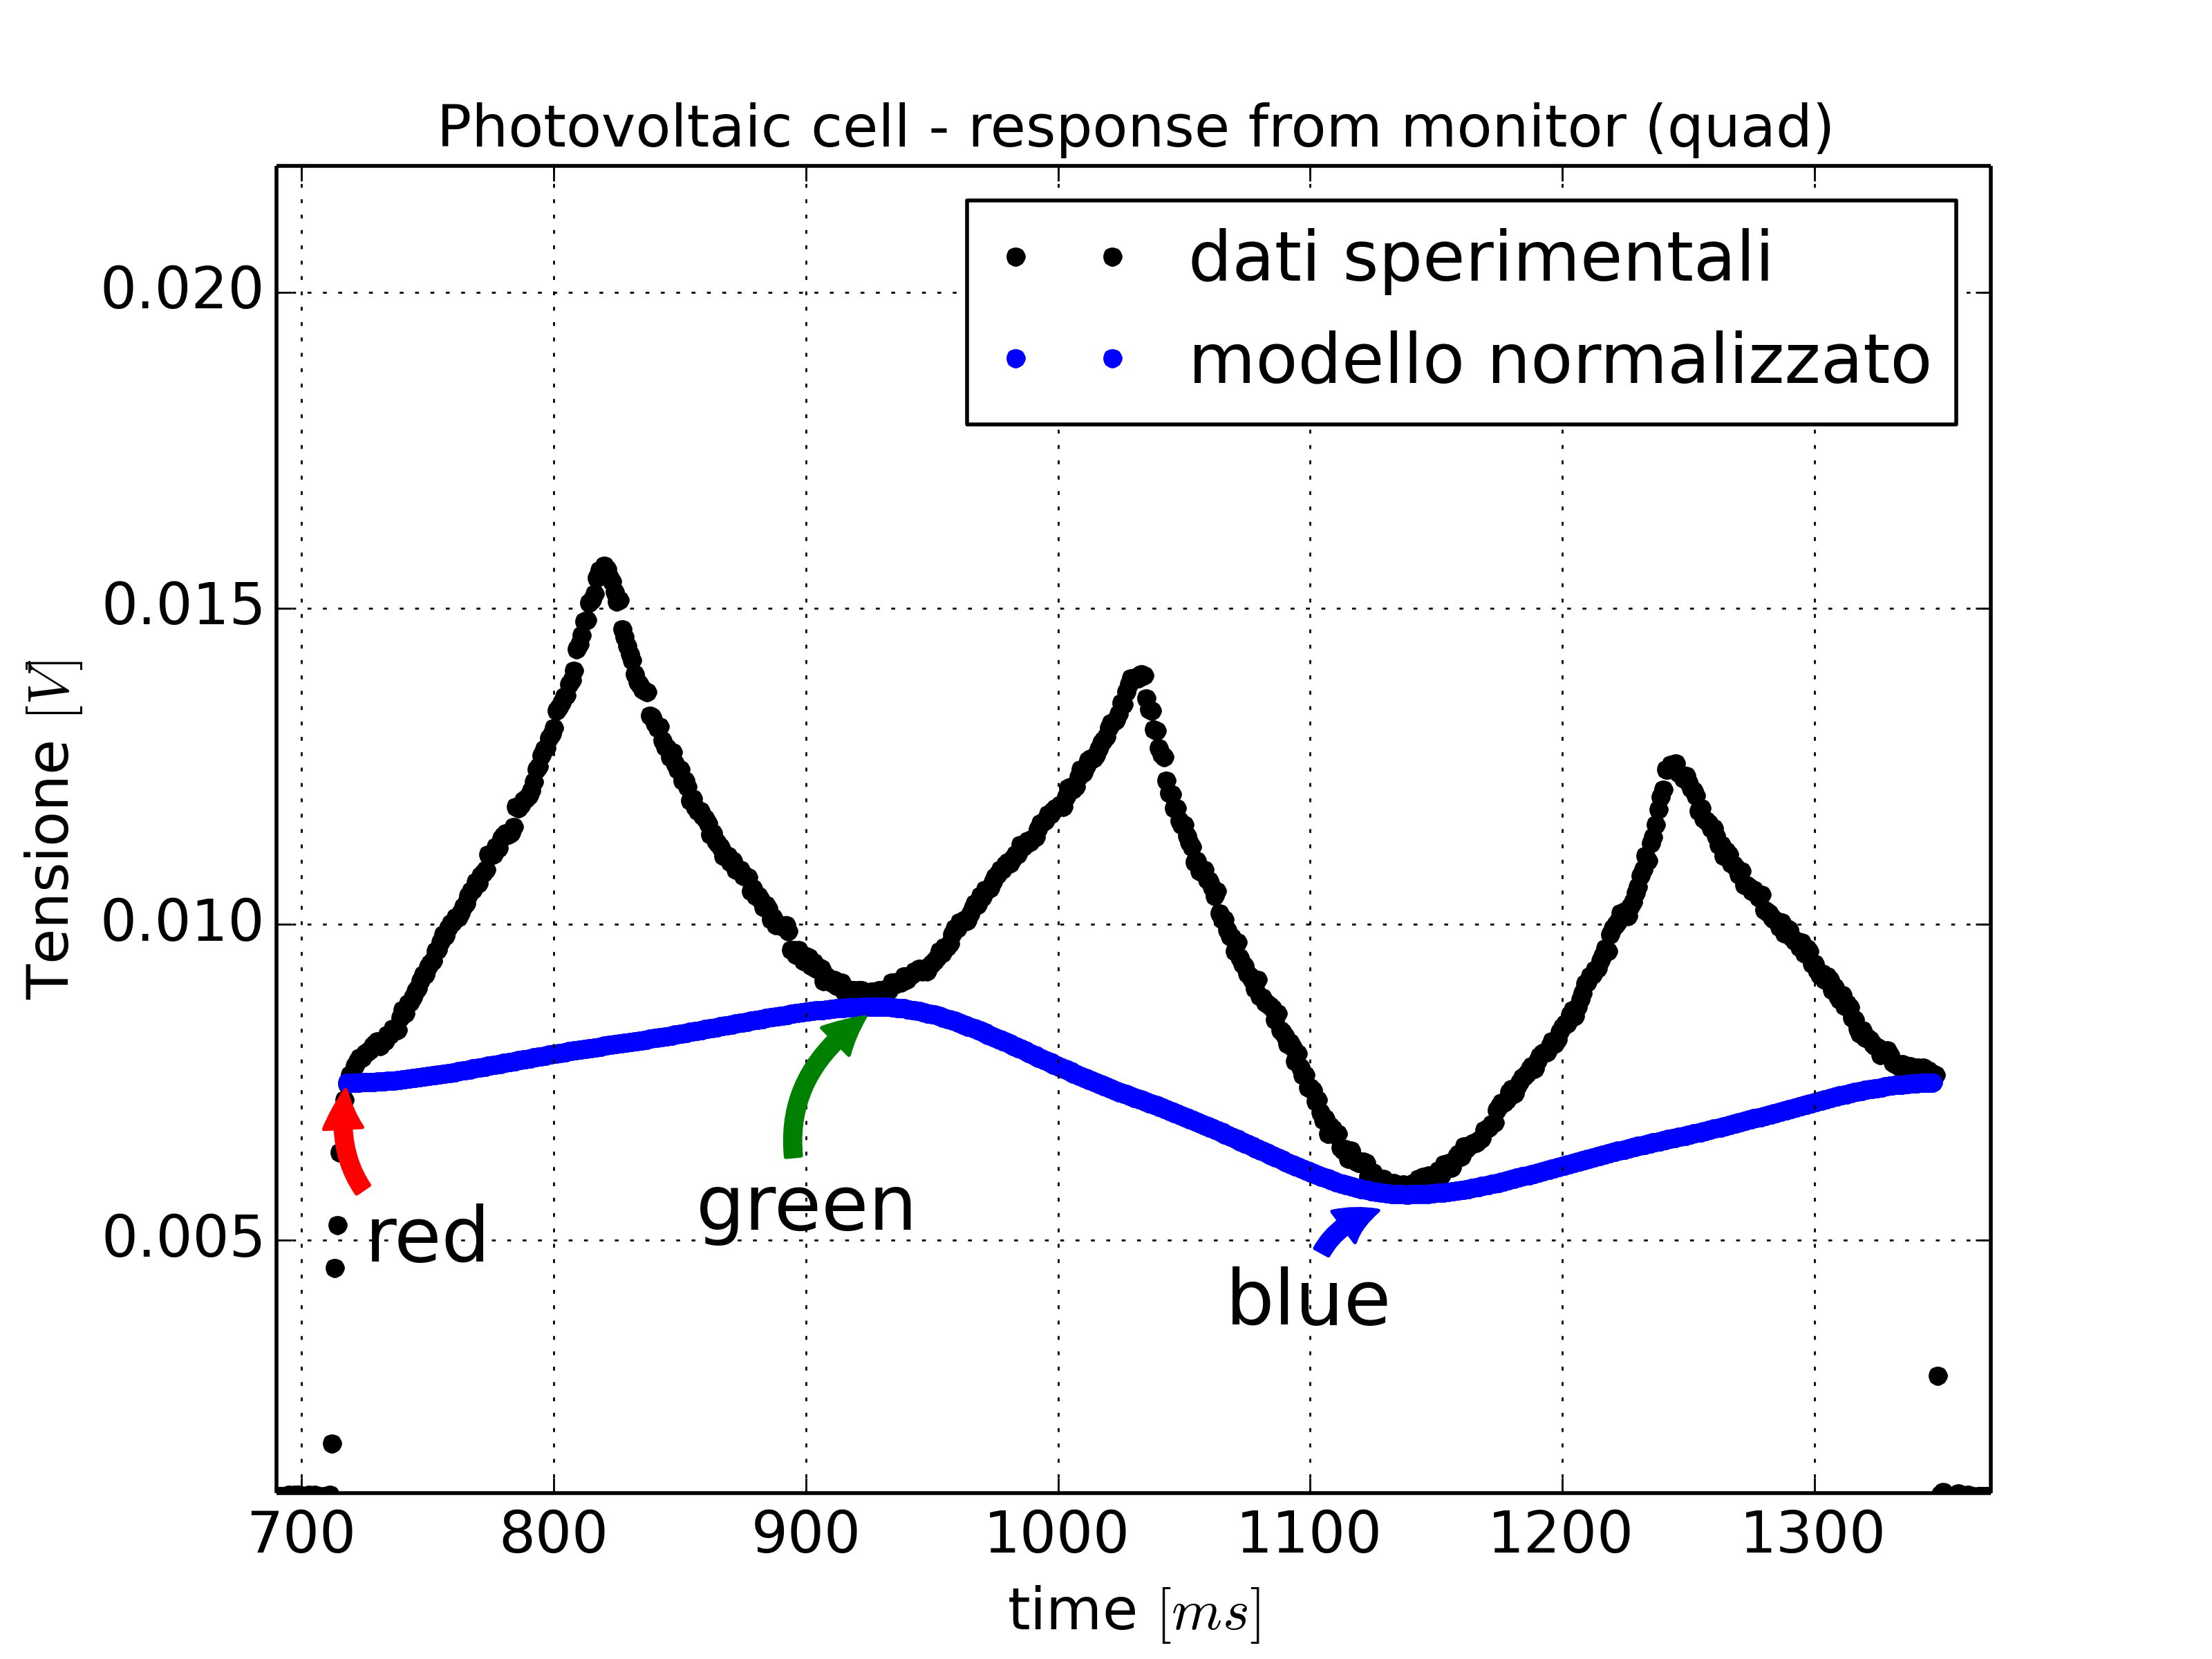
\includegraphics[width=0.55\linewidth]{./dati_normal}
\end{figure}

\begin{itemize}
\item Con il modello quadratico avevamo ricavato le intensità relative dei colori puri.
\item Adesso siamo in grado di assegnare un valore di "pseudo-wavelength" per ogni tripletta.
\end{itemize}

\end{frame}

\begin{frame}{Coincidenze? Noi crediamo di no.}

\begin{textblock}{12}(-1.5,4)
\begin{figure}
\centering
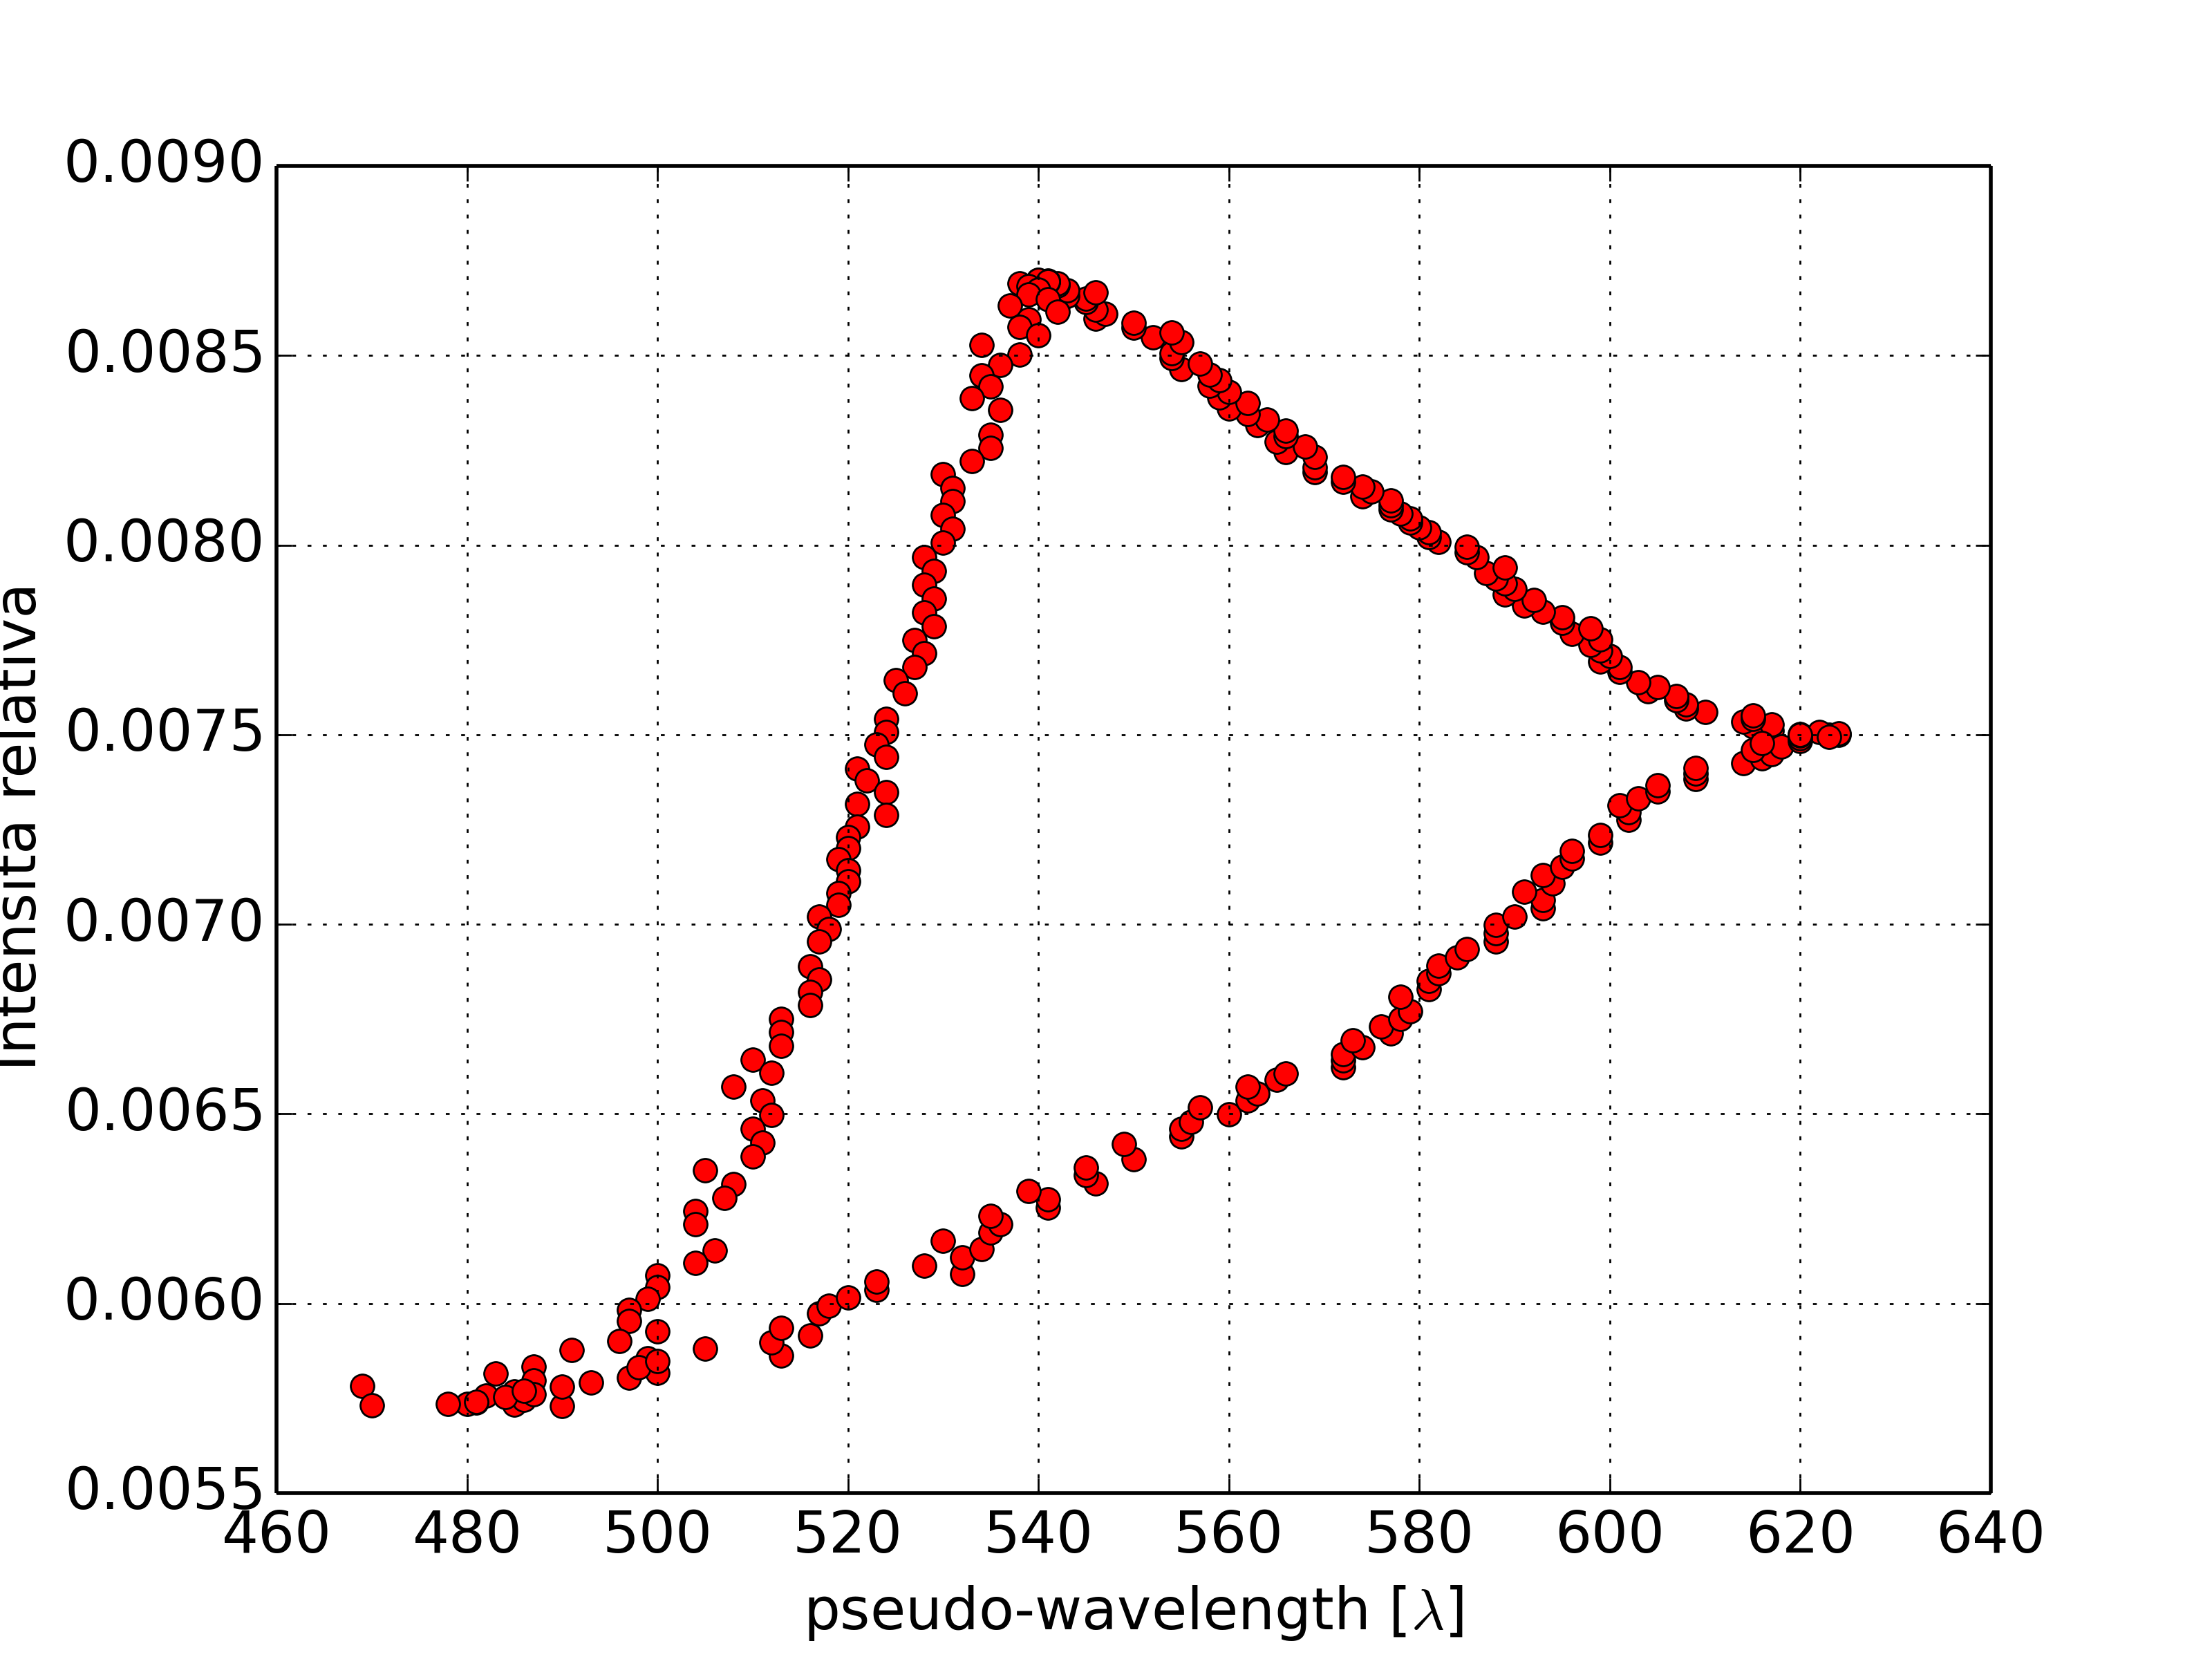
\includegraphics[width=0.7\linewidth]{./nostro_gamut}
\label{fig:nostro_gamu}
\end{figure}
\end{textblock}


\begin{textblock}{12}(6,4)
\begin{figure}
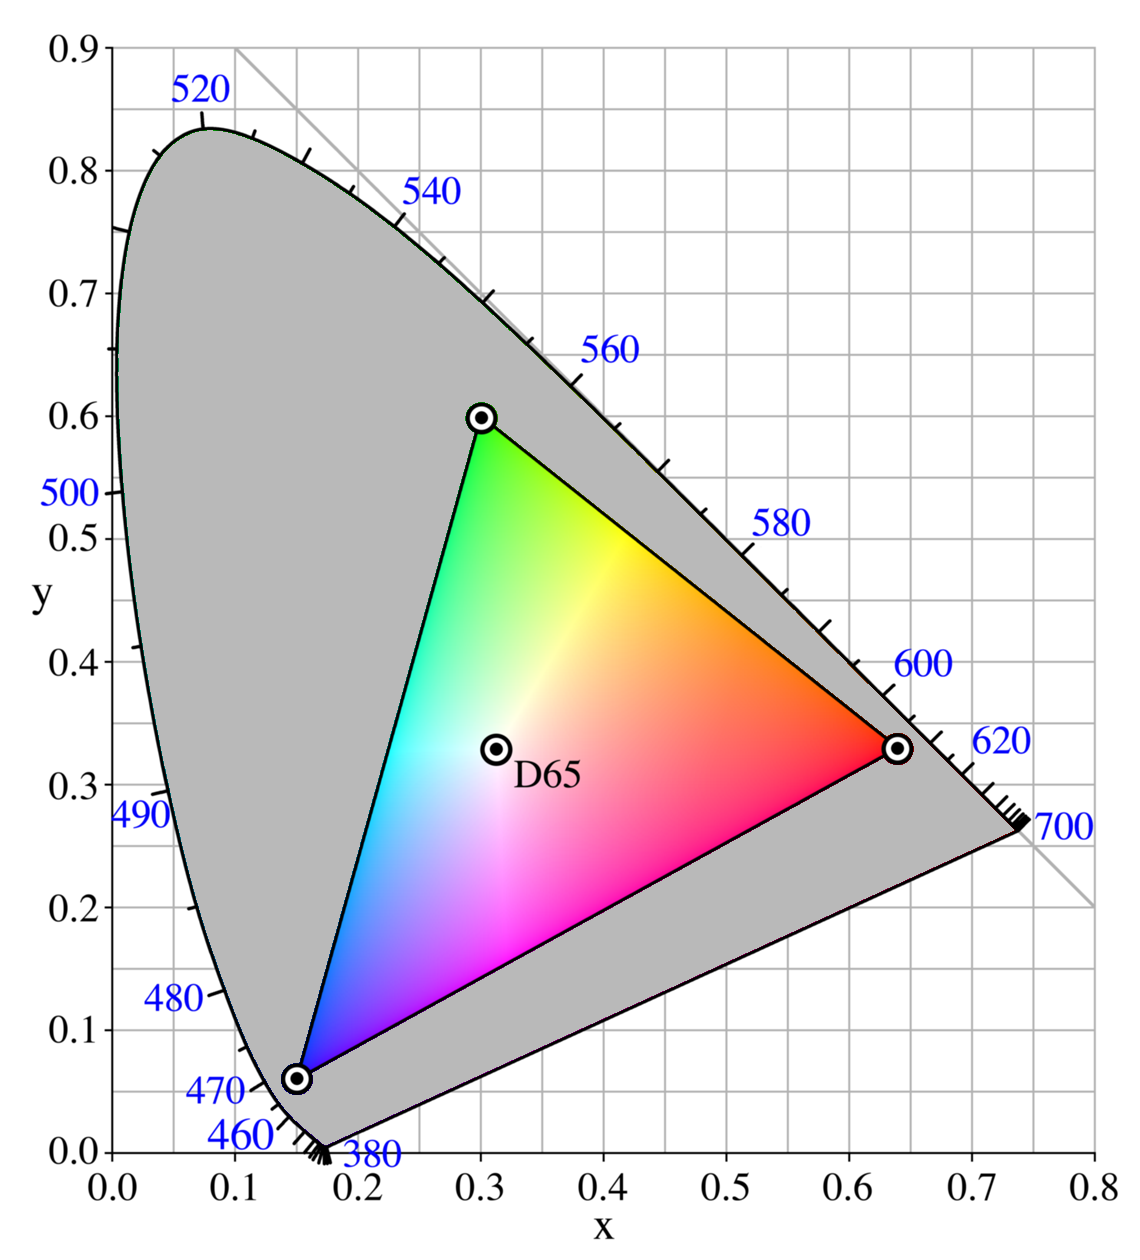
\includegraphics[width=0.45\linewidth]{./8_CIExy1931_sRGB_gamut_D65}
%\label{fig:cal}
\end{figure}
\end{textblock}



Noi crediamo di no.

\end{frame}

\begin{frame}
\begin{itemize}
\item Nel nostro grafico l'asse y corrisponde alla luminosità relativa dei colori $\leftrightarrow$ asse y del gamut.
\item L'asse x del gamut è una misura di quanto rosso è presente nella radiazione e questa quantità aumenta andando da sinistra a destra. Incidentalmente la nostra pseudo lunghezza d'onda classifica a sua volta i colori RGB in base allo stesso criterio poichè procedendo verso $\lambda$ maggiori ci avviciniamo al colore rosso.
\item Con questo non vogliamo dire le le scale coincidono, ma che è possibile stabilire fra le due una certa corrispondenza qualitativa.
\end{itemize}
\end{frame}

\end{document}